\section{EVALUATION }
\label{section:results}
This section presents a thorough evaluation of our LPSBL system.
In the first half of this section, we evaluate the parameters that affect the localization performance of LPSBL.
In the second half of this section, test-bed experiment is carried out in indoor environments to verified the localization ability of the LPSBL system.

\subsection{Simulation}
We develop a Monte Carlo simulator to evaluate the localization performance under different conditions.
In the simulation, the nodes are randomly deployed in a field of $10m \times 10m$. 
Considering the impact of the uncertainty of node position and TOA detection, we add a certain amount of node location error and TOA measure error in all the simulations.
All the statistics are running more than 100 times for high confidence, and reported by RMSE figure. 
Table 1 illustrates the default simulation setup parameters.
\begin{table} [!h] \normalsize
\caption {\textbf{Default configuration parameters}} %title of the table
\centering % centering table
    \begin{tabular}{|c|c|}
        \hline
Parameter & Description \\
 \hline
Field Area & 10m $\times$ 10m \\
\hline
Number of Anchors & 20 (Default) \\
 \hline
Position Error of Nodes	 & 0.05m (Default) \\
 \hline
TOA Detection Error 	 & 0.50ms (Default) \\
 \hline
Random-Seed Loop	 & 500 times (Default) \\
 \hline
Error Statistics	 &  RMSE \\
        \hline
    \end{tabular}
\end{table}

The results of simulation evaluation are as following:

\textbf{1) Impact of the number of nodes:}
 In this experiment, we investigate the localization error and number of anchors with a different number of anchors from 10 to 40 in steps of 2. 
 We run the simulation with the TOA error is 0.1ms, and other simulation parameters are default. 
 With more anchors, the whole area will be divided into smaller parts, 
 thus more accurate localization estimation should be achieved in the three methods. 
Figure \ref{Nodenumbers} confirms our expectation. As shown in Fig. \ref{Nodenumbers}, with the number of anchors increases, localization error for both  methods are down slowly. 
Figure \ref{Nodenumbers} also shows that the localization error of the LPSBL method is approximate to the SBL method when the number of anchor node is larger.
  \begin{figure}[htb]
            \setlength{\abovecaptionskip}{0pt}
            \centering
			 \vspace{-3mm}
           		 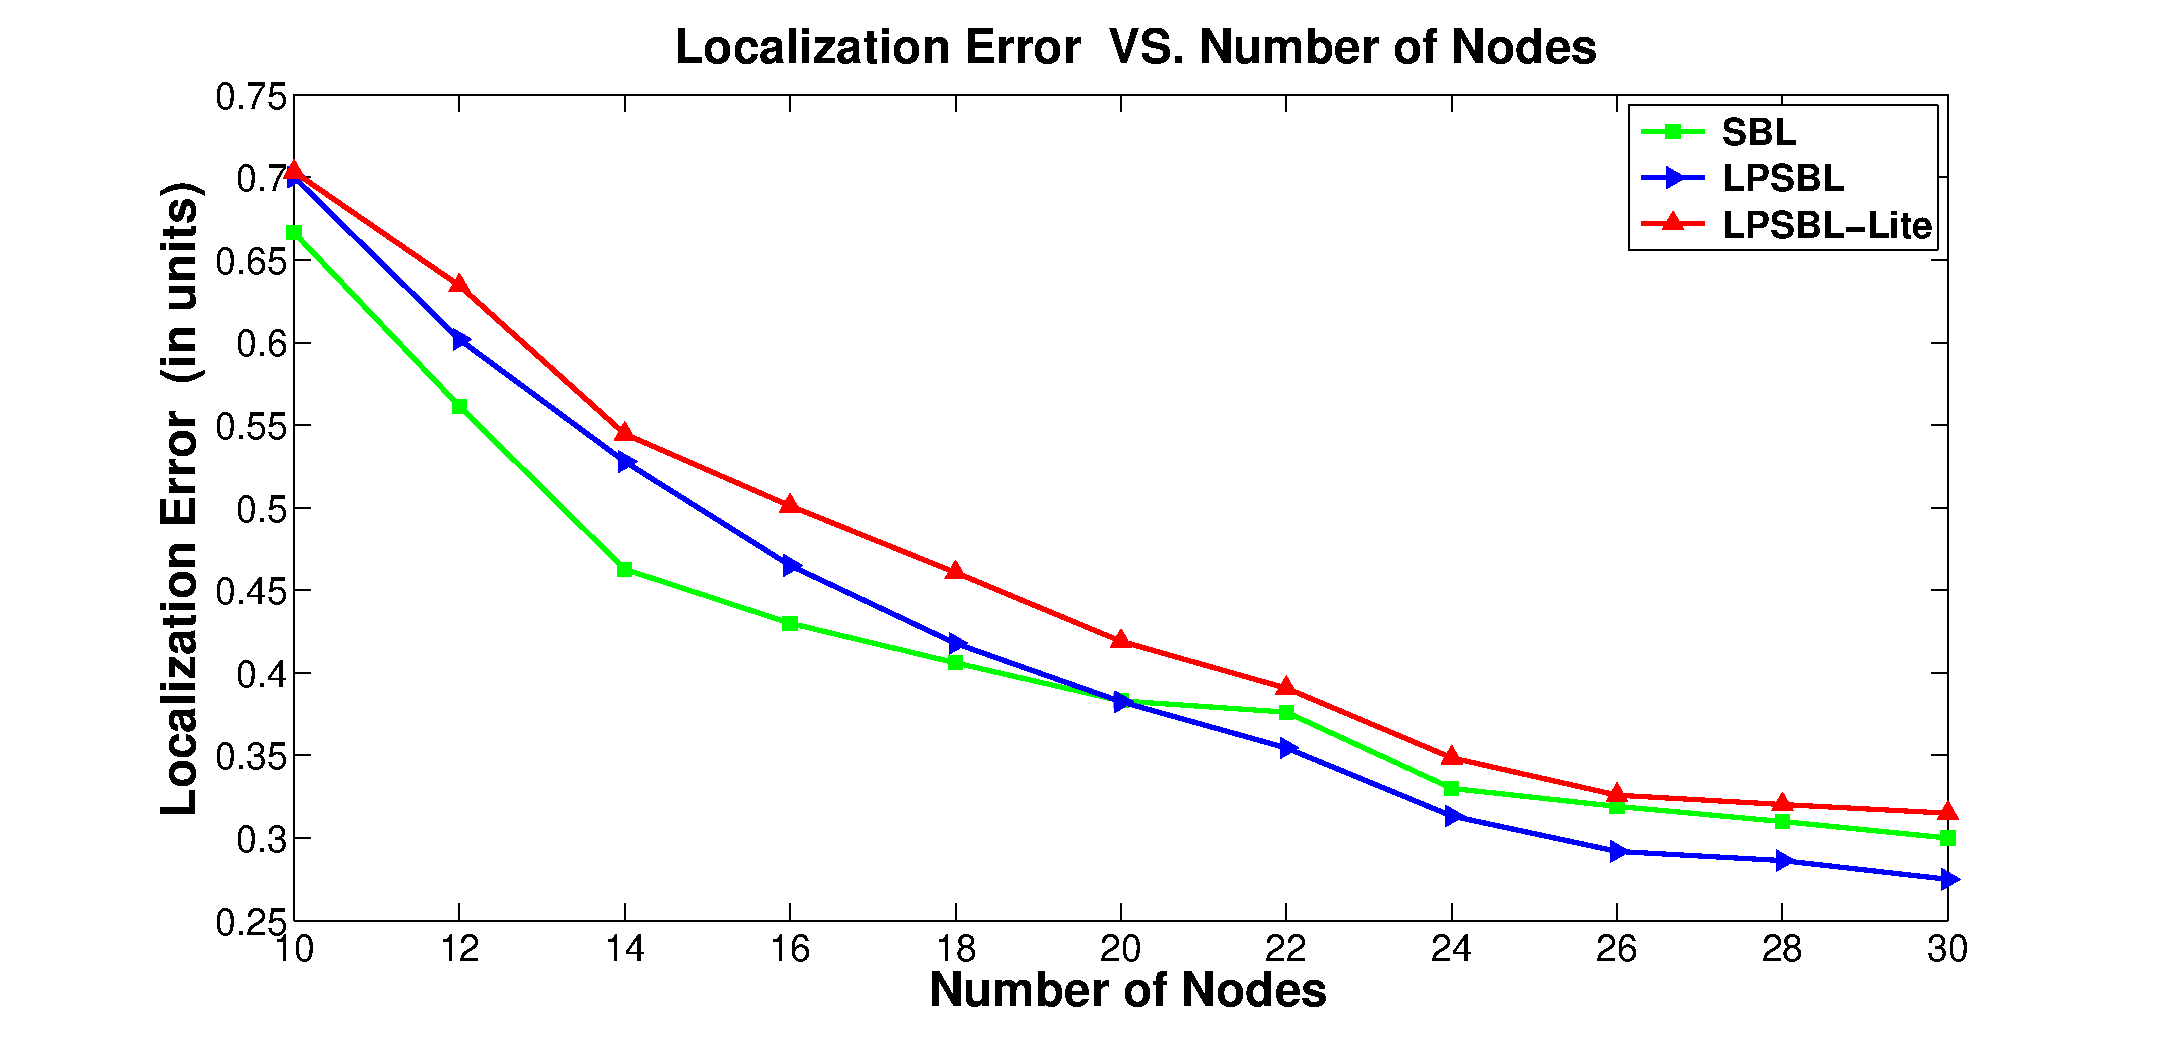
\includegraphics[height=5.0cm,width=7.0cm]{image/Nodenumbers.eps}
           % \vspace{15mm}
            \caption{Localization Error vs. Number of Nodes}
             \vspace{-5mm}
             \label{Nodenumbers}
        \end{figure}	
		
\textbf{2) Impact of the position errors of nodes:}
 In this experiment, we compare the two methods for different position errors of anchors. 
 In Fig. \ref{fig5}, we choose the position error with the range from 0 to 0.4m in step of 0.02m for the two methods. 
 Fig. \ref{fig5} indicates the position error of anchors has an effect on the localization results. 
 For the both methods, the localization error increases as position error increases in Fig. \ref{fig5}. 
 The localization performance of LPSBL is better than SBL when the position errors of nodes is less than 0.4m.
 %which demonstrates the LPSBL method is the most robust to the node position error.
  \begin{figure}[htb]
            \centering
		   \vspace{3mm}
			 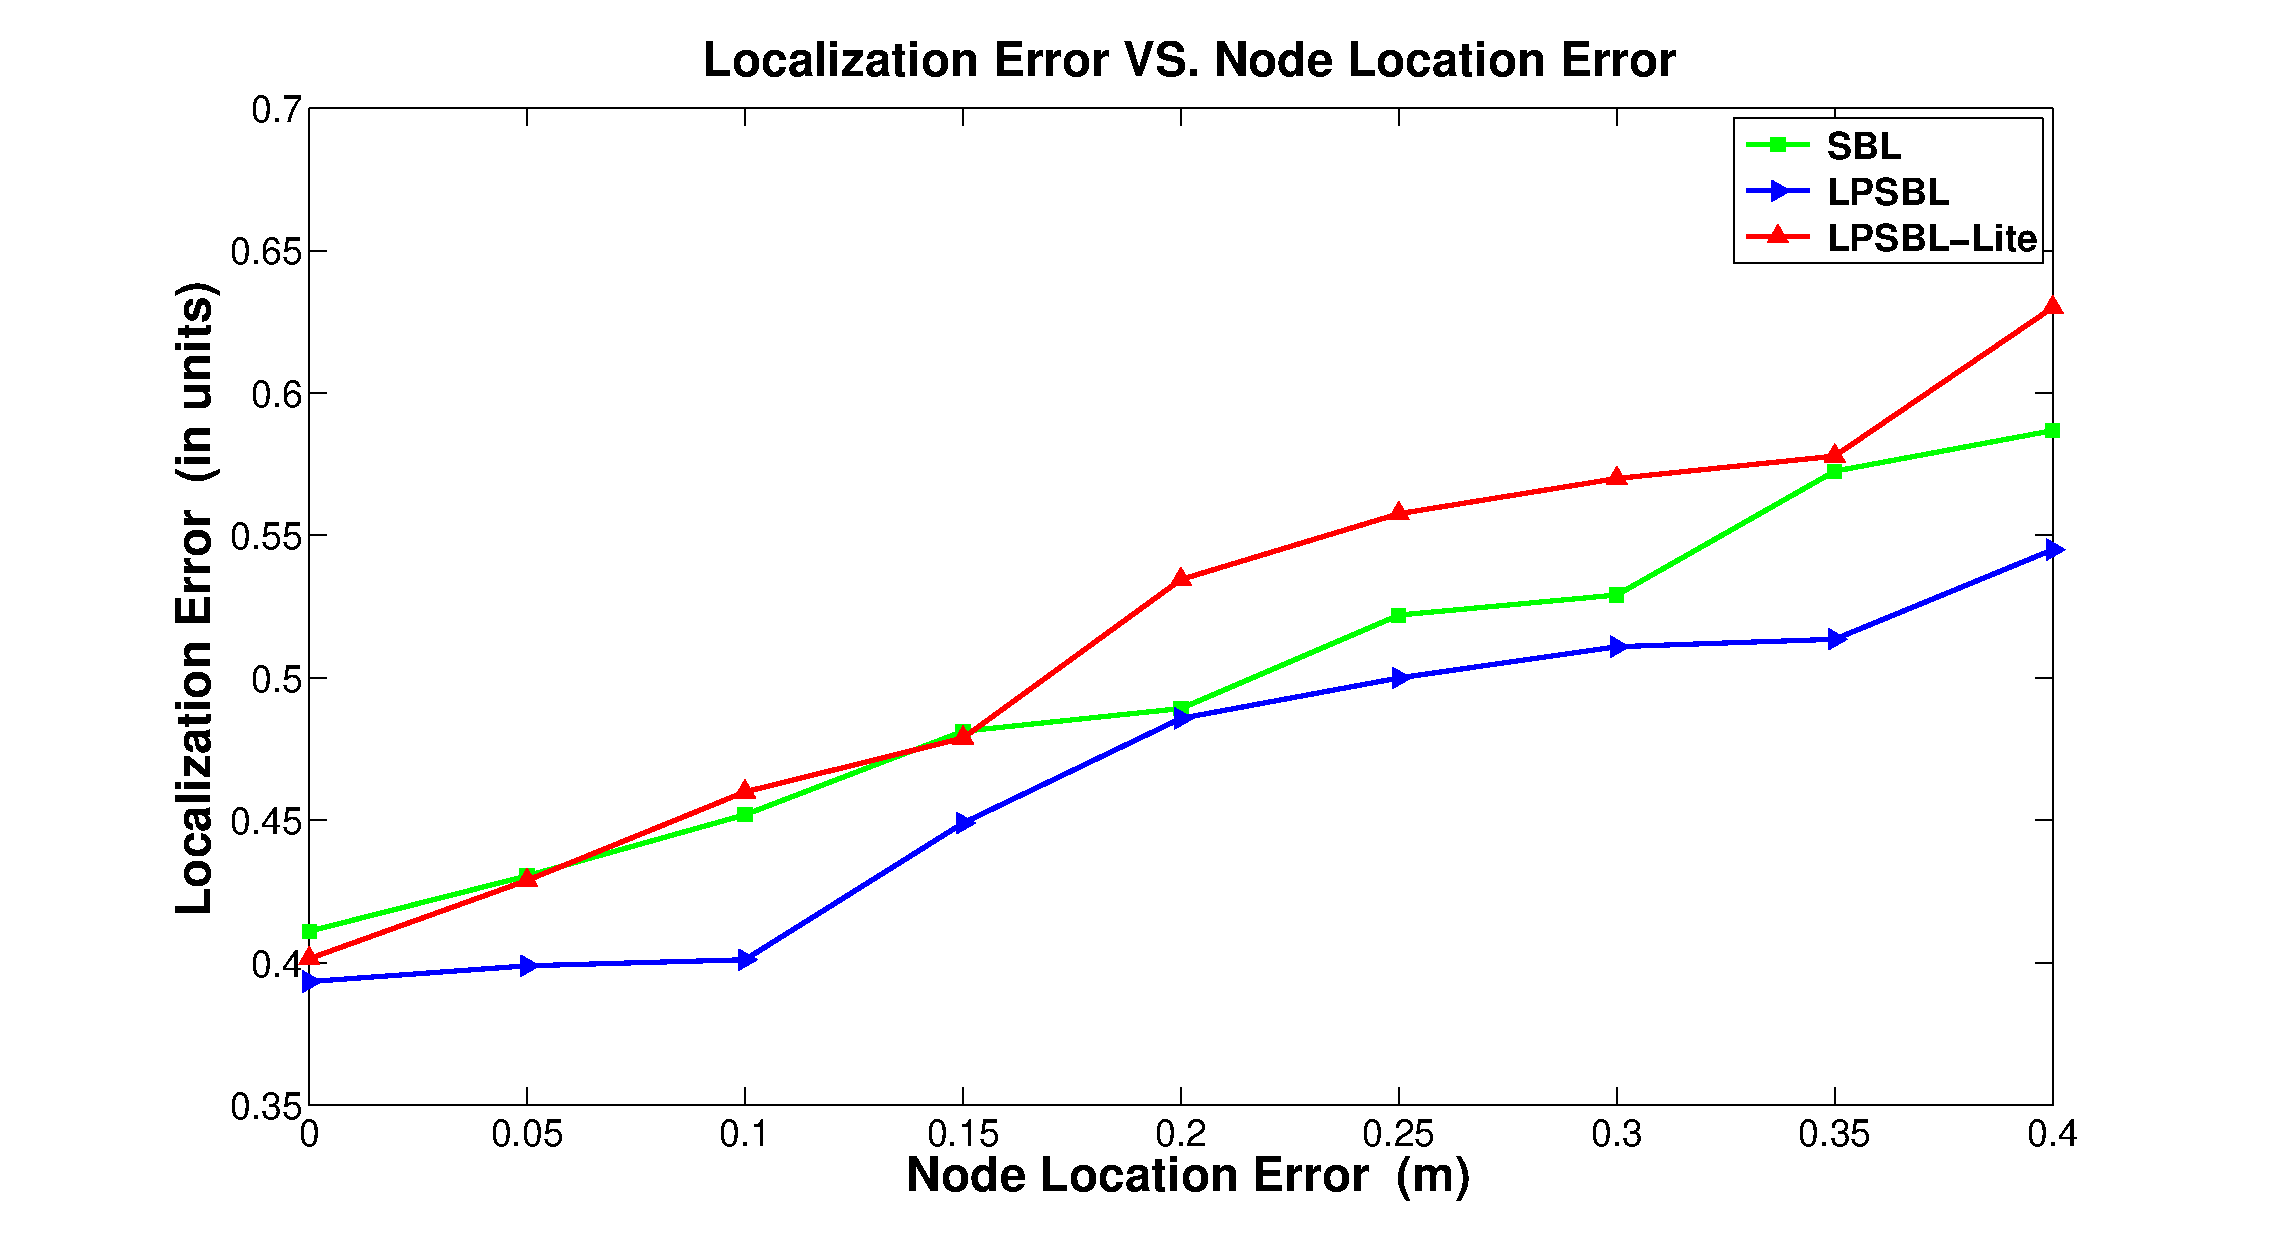
\includegraphics[height=5.0cm,width=7.0cm]{image/locationerror.eps}
              \caption{Localization Error vs. Node Position Error}
             \vspace{-5mm}
             \label{fig5}
        \end{figure}

\textbf{3) Impact of the TOA measurement error:}
In this experiment, we discusses the impact of the TOA error of nodes for several methods being compared with the range from 0 to 2ms in steps of 0.1ms. 
Other simulation parameters keep default. 
Figure \ref{fig6} reports the average localization error of both localization methods. 
Results clearly show a significant increases of the localization error as increases of TOA measurement error.
In conclusion one can observe that the error of TOA measurement has significant influence on the localization accuracy. 
%Also, the LPSBL method has a better result than the SBL method. 
%It is shown in Fig. \ref{fig6}, the localization error of our LPSBL method is stable no matter which degree the TOA error is, which means that the LPSBL method can localize the target node with little error when TOA error is not too big.
  \begin{figure}[htb]       
            \centering
			\vspace{-3mm}
            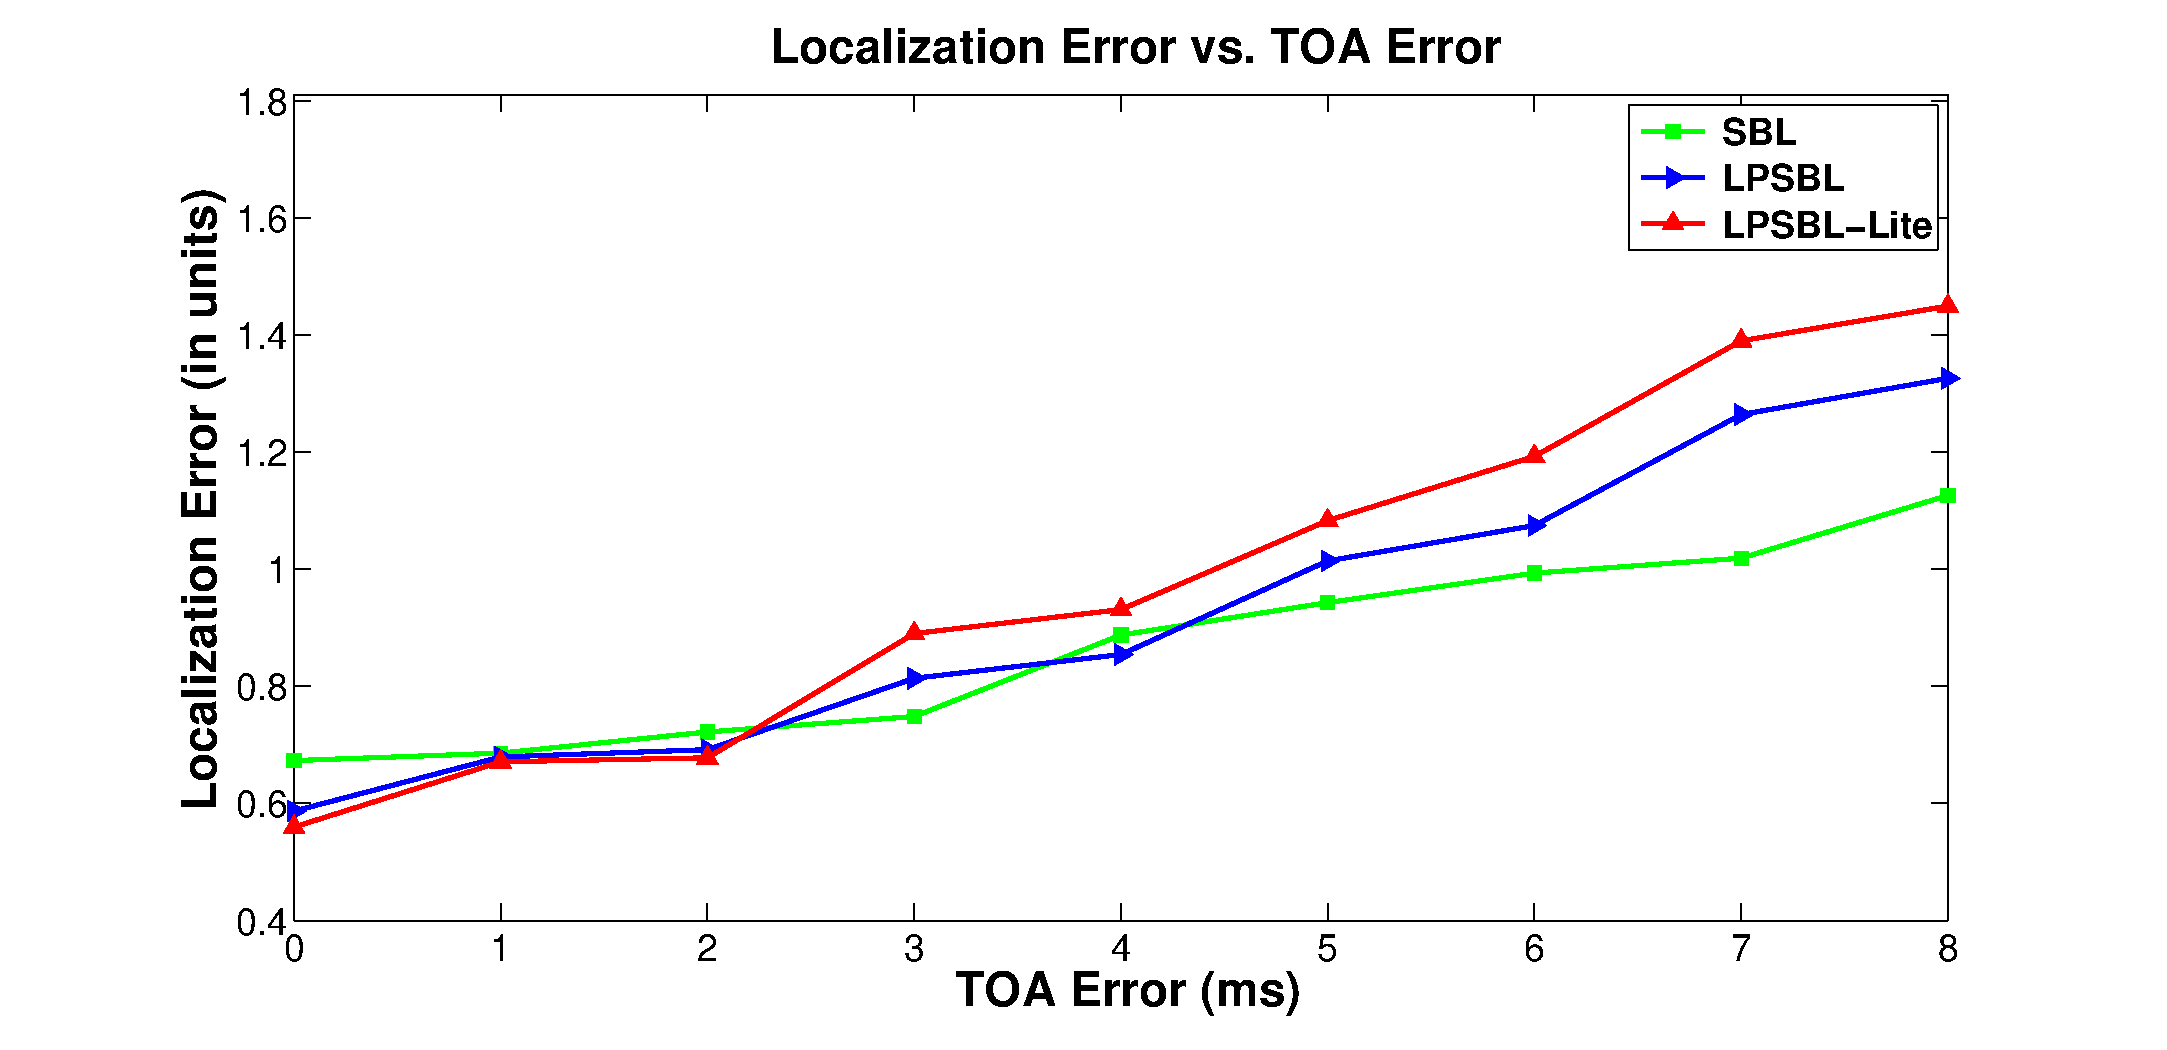
\includegraphics[height=5.0cm,width=7.0cm]{image/TOA.eps}
                \caption{Localization Error vs. TOA Error}
             \vspace{-8mm}
             \label{fig6}
        \end{figure}
	 % \textbf{Summary:} From the above simulations, considering the different factors, including the number of anchors, the node position error and TOA measurement error of the anchors, we can get the following conclusions:
 % (1) With increasing number of the number of anchors, localization errors decrease for both methods, and LPSBL has better localization performance;
 % (2) The error of node position can impact the localization error, the proposed LPSBL method is more robust to the error of node position than SBL method;
  % (3) The TOA measurement error has a major impact on the localization accuracy, and the proposed LPSBL method can achieve better localization performance.

  
 \subsection{Result of Incremental LPSBL}
 In this simulation, we discuss the performance of incremental LPSBL.
We investigate the localization error and number of anchors with a different number of anchors from 10 to 40 in steps of 2. 
 We run the simulation with the TOA error is 0.1ms, and other simulation parameters are default. 
 Figure \ref{Incremental} reports the average localization error of localization methods. 
 Compared with the LPSBL, the localization performance of incremental LPSBL is slightly decreased.
 
    \begin{figure}[htb]       
            \centering
			\vspace{-3mm}
            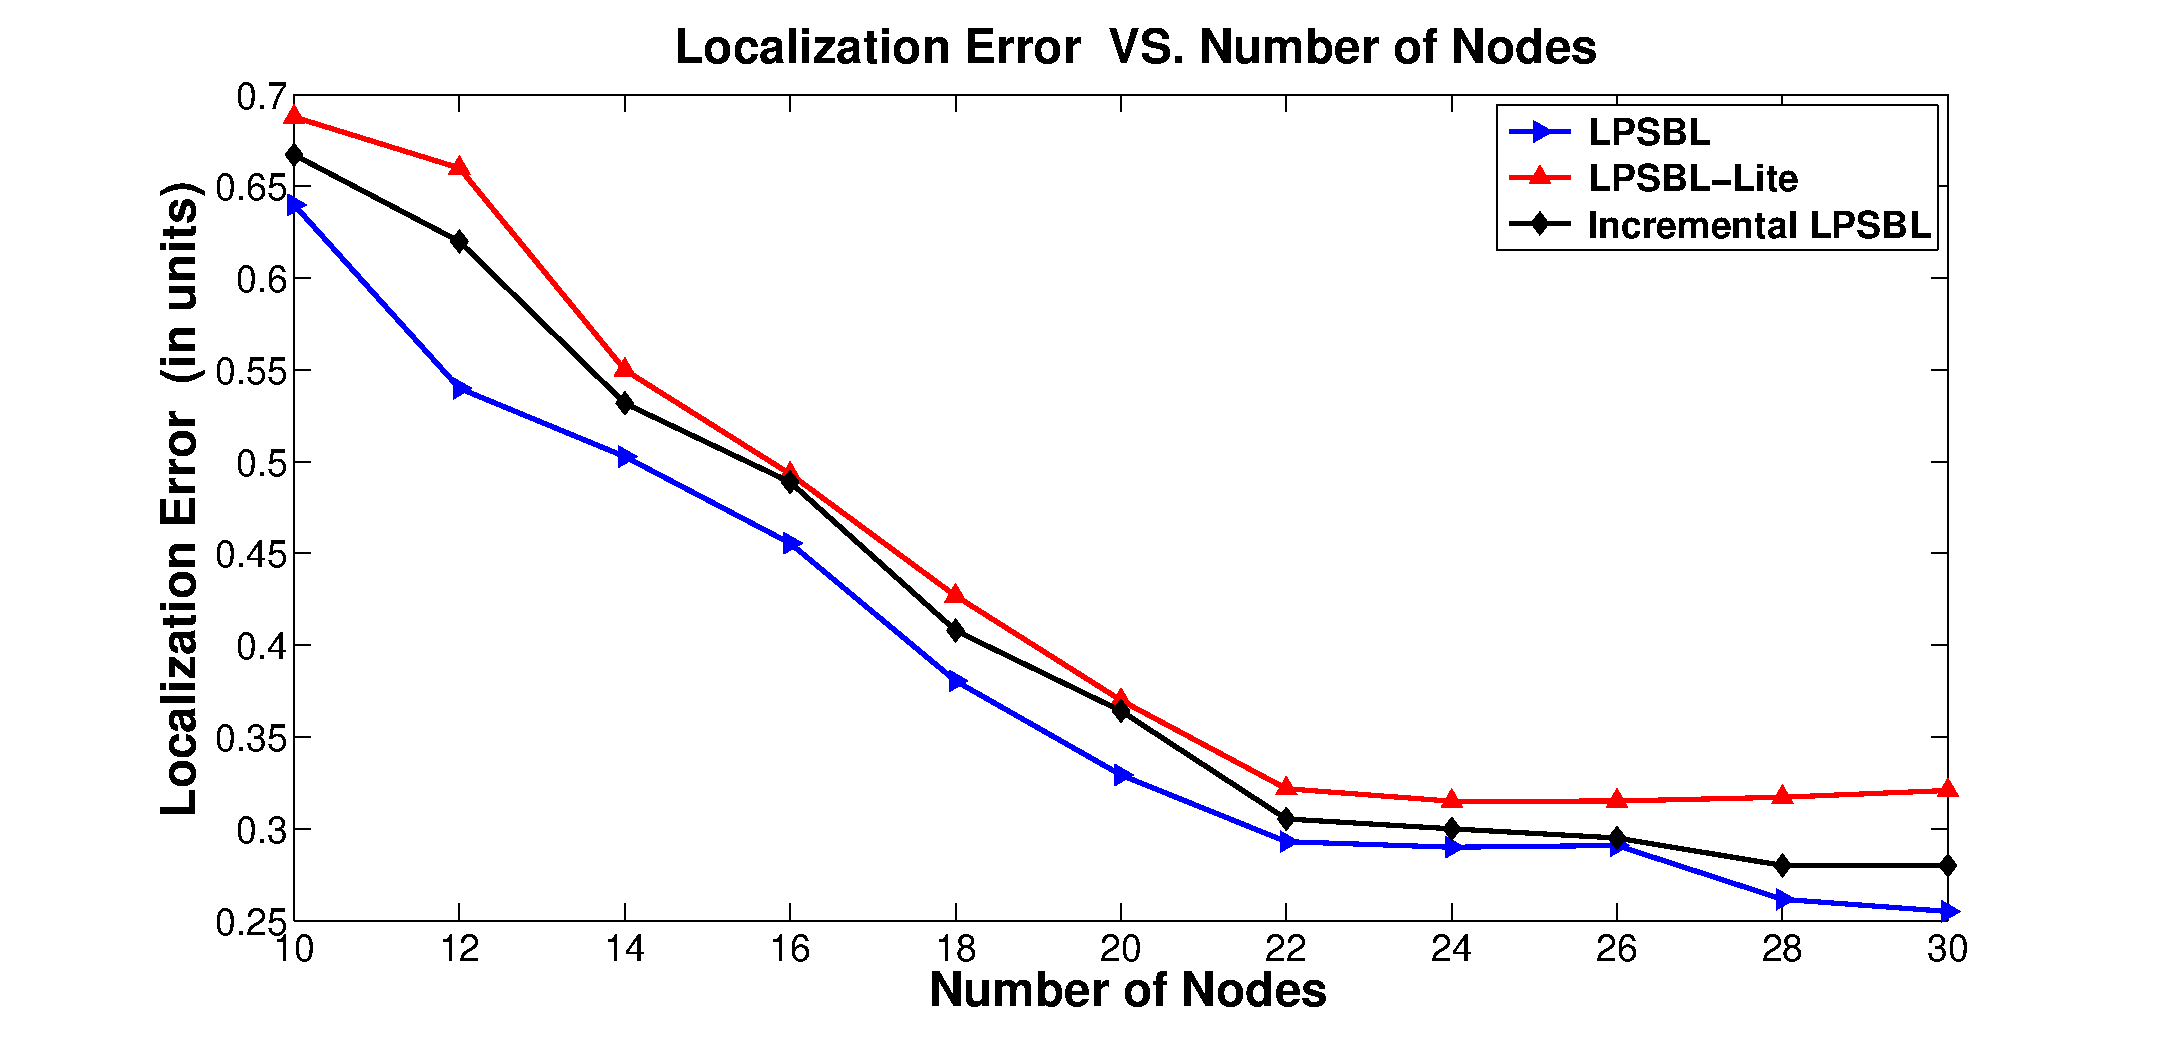
\includegraphics[height=5.0cm,width=7.0cm]{image/Incremental.eps}
                \caption{Localization Error vs. TOA Error}
             \vspace{-8mm}
             \label{Incremental}
        \end{figure}
		


  \subsection{Emulation}

In this section, we evaluate the localization performance of LPSBL system in our test-bed.
we use 30 Samsung smartphones as anchors and connect them through CISCO CVR328W-K9-CN wireless router. 
TPSN protocol is adapted in the proposed LPSBL system to realize time synchronization.
The 30 smartphones are randomly deployed in a size of 16m$\times$10m space and there just one dominating acoustic source during an experiment.
In the experiment, smartphones are random deployed in the space, and 100 times localization results are shown in Fig.~\ref{emulation}. 
In the figure, blue squares stand for smartphones, red circle squares are the real position of acoustic sources, and black dot are the estimated location by LPSBL. 
An arrow origins from the estimated location of each acoustic source and points to its real position. 
As the results shown in Fig.~\ref{emulation}, most of estimated locations of the acoustic sources are close to the ground truth.
The localization errors are very small except some point near the bound of network, it is normal for the SBL-type methods.
The experiments of test-bed shows that LPSBL can effectively localize the acoustic source in the practical application.
  \begin{figure}[htb]
         %    \centering
			%\vspace{-3mm}
            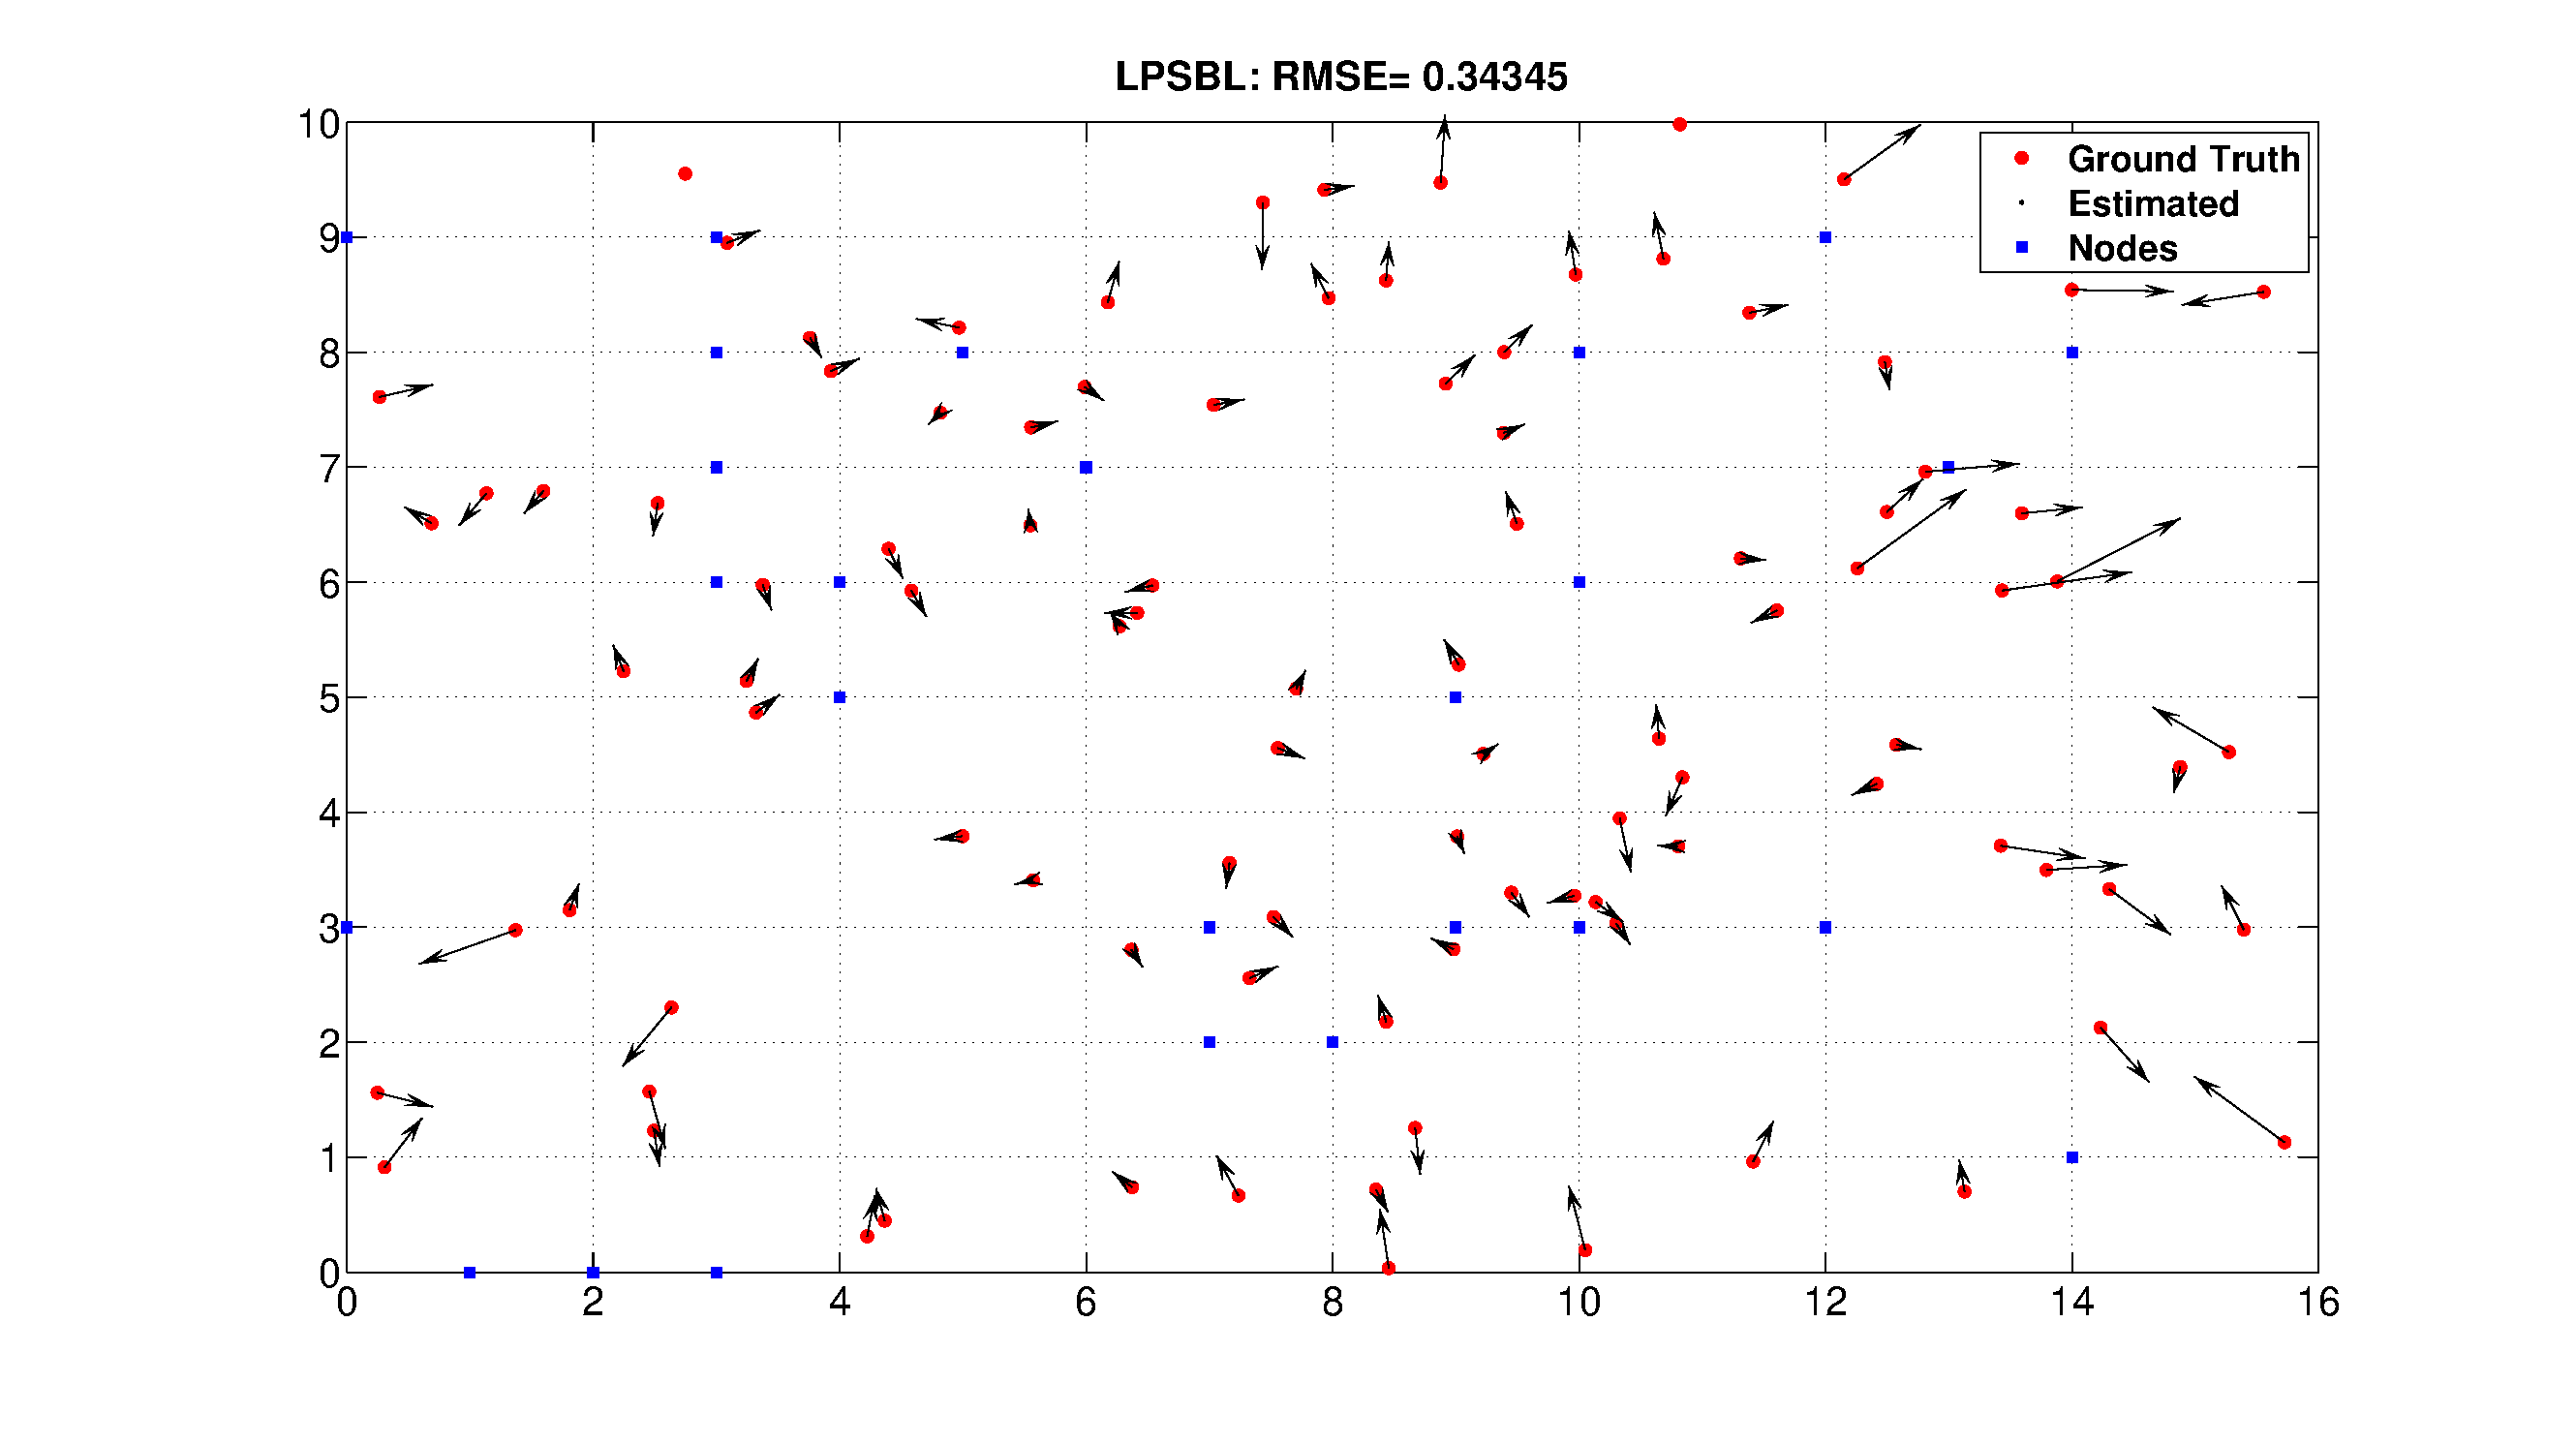
\includegraphics[height=6cm,width=9.0cm]{image/emulation.eps}
             \caption{Test-bed localization result of the proposed LPSBL}
             \vspace{-5mm}
             \label{emulation}
        \end{figure}
